\begin{frame}{Triangle construction}
\begin{enumerate}
\conti
\item Construct an isosceles triangle in which the lengths of the equal sides is 6.5 and the angle between them is 110$\degree$
\seti
\end{enumerate}
\begin{itemize}
\item\textbf{Solution}\\
\begin{tikzpicture}
[scale =0.6,>=stealth,point/.style = {draw, circle, fill = black, inner sep = 1pt},]
\node (B) at (0,0)[point,label=below :$B$] {};
\node (A) at (-2.223,6.108)[point,label=above :$A$] {};
\node (C) at (6.5,0)[point,label=below :$C$] {};
\draw (A)--(B);
\draw (B)--(C);
\draw (C)--(A);
\tkzMarkAngle[fill=green!40,size=0.5cm,mark=](C,B,A)
\tkzLabelAngle[pos=1](C,B,A){\rotatebox{-360}{$110$}}
\end{tikzpicture}

\item BC = 6.5 \item AC = 10.64
\item AB = 6.5\\
\item $\angle B$ = 110\\ 
\end{itemize}
\end{frame}
\begin{frame}
\begin{itemize}
\item\textbf{Given}: BC = 6.5 and AB = 6.5\\
$\angle$ABC = 110
\begin{align*}
a = 6.5 and  c = 6.5\\
b = \sqrt{a^2 + c^2 - 2ac cos(A)}\\
b= 10.64\\
p=\frac{a^2 + c^2 - b^2}{2a}\\
p=-2.22\\
q=\sqrt{c^2 - p^ 2}\\
q = 6.10
\end{align*}
\end{itemize}
\end{frame}

\begin{frame}
\begin{figure}
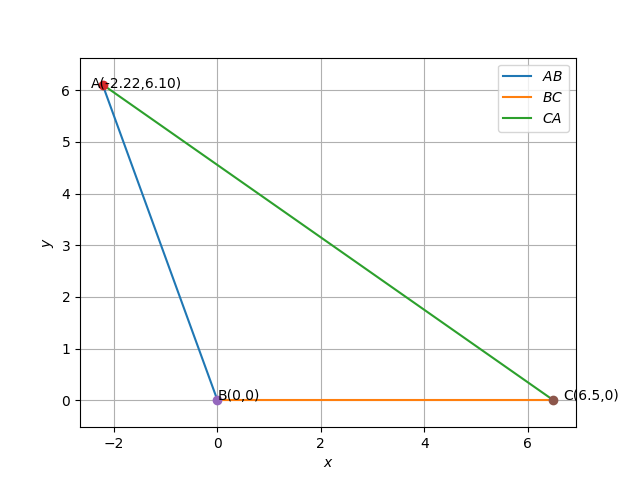
\includegraphics[scale=.4]{./CODES/triangle/TRI_CON.png}
\end{figure}
\begin{itemize}
\item \url{https://github.com/pratibha444/GEOMETRY/blob/master/figs/tri_iso.tex}
\item \url{https://github.com/pratibha444/GEOMETRY/blob/master/CODES/triangle/TRI_CON.py}
\end{itemize}
\end{frame}